% -----------------------------------------------------
% By Jonathan C. Roberts
% File modified: 15.01.2003 - nb29
% -----------------------------------------------------
\documentclass[twocolumn]{article}

 \usepackage[utf8]{inputenc}
\usepackage{times}
\usepackage{graphicx}
\usepackage{wrapfig}
\usepackage{caption}
\usepackage{subfig}
\usepackage{lipsum}
\usepackage{enumitem}
\usepackage{color}
\usepackage{csquotes}
\usepackage[hidelinks,draft]{hyperref}
\usepackage[]{units}

\graphicspath{{figures/}}
\DeclareGraphicsExtensions{.pdf,.png}

%set dimensions of columns, gap between columns, and paragraph indent
\setlength{\textheight}{8.75in}
\setlength{\columnsep}{2.0pc}
\setlength{\textwidth}{6.8in}
%\setlength{\footheight}{0.0in}
\setlength{\topmargin}{0.25in}
\setlength{\headheight}{0.0in}
\setlength{\headsep}{0.0in}
\setlength{\oddsidemargin}{-.19in}
\setlength{\parindent}{1pc}

\setlength{\parskip}{0.25pc} % very ugly without it... (DL)

\makeatletter
%to get 12 point spacing for normalsize text, must set it to 10 points
\def\@normalsize{\@setsize\normalsize{10pt}\xpt\@xpt
\abovedisplayskip 10pt plus2pt minus5pt\belowdisplayskip
\abovedisplayskip \abovedisplayshortskip \z@
plus3pt\belowdisplayshortskip 6pt plus3pt
minus3pt\let\@listi\@listI}

%need an 10 pt font size for subsection and abstract headings
\def\subsize{\@setsize\subsize{10pt}\xipt\@xipt}

%make section titles bold and 12 point, 2 blank lines before, 1 after
\def\section{\@startsection {section}{1}{\z@}{1.0ex plus
1ex minus .2ex}{.2ex plus .2ex}{\large\bf}}

%make subsection titles bold and 11 point, 1 blank line before, 1 after
\def\subsection{\@startsection {subsection}{2}{\z@}{1.2ex
plus 1ex}{.2ex plus .2ex}{\subsize\bf}}

\def\keywords{\vspace{.6em}
    \if@twocolumn
	\small{\itshape Keywords\/}\bfseries---$\!$%
    \else
	\small{\itshape Keywords\/}\bfseries---$\!$%\end{center}\quotation\small
      %\begin{center}\small\bfseries Keywords\end{center}\quotation\small
    \fi}
\def\endkeywords{\vspace{0.6em}\par\if@twocolumn\else\endquotation\fi
    \normalsize\rm}
    
\usepackage{ifthen}
\newboolean{blinded}
\setboolean{blinded}{false}

\renewcommand{\sectionautorefname}{Section}
\renewcommand{\figureautorefname}{Fig.}

\newcommand*{\eg}[1]{{e.g.}, #1}
\newcommand*{\Eg}[1]{{E.g.}, #1}
\newcommand*{\ie}[1]{{i.e.}, #1}
\newcommand*{\ia}[1]{{inter~alia}, #1}
\newcommand*{\etal}{{et~al.} }	
\newcommand*{\wrt}{{with respect to} } %w.r.t.

\newcommand{\pprelim}[1]{\color[rgb]{0.08,0.32,0.64}#1}
\newcommand{\ptodo}[1]{\color[rgb]{0.64,0.08,0.32}#1}

% custom teaser command \teaser{imagefile}{cpation}
\newcommand{\teaser}[2]{
	\newcommand{\@teasergraphics}{#1}
	\newcommand{\@teasercaption}{#2}}

\newcommand\titlefig{%
	\\[\normalbaselineskip]\hspace{-9pt}
	\begin{minipage}[t]{\linewidth}
		\includegraphics[width=\linewidth]{\@teasergraphics}\\
		\refstepcounter{figure}\normalsize{Figure~\thefigure: \@teasercaption}
		\label{fig:teaser}
	\end{minipage}}

\makeatletter
\patchcmd\@maketitle{\LARGE\@title}{\Large\textbf{\@title}}{}{}
\patchcmd\@maketitle{\@author}{\@author\titlefig}{}{}
\makeatother

\usepackage{eso-pic}
\AddToShipoutPictureFG{\AtPageLowerLeft{\put(\LenToUnit{0.5\paperwidth},\LenToUnit{6mm}){\makebox[0pt][c]{\fontsize{6.5}{8}\selectfont\color[gray]{0.5}Author's revised version (2026-11-14). Version of record: \url{https://doi.org/10.1109/IV.2016.61}}}}}
\begin{document}

\title{Evaluation of Sketchiness as a Visual Variable for 2.5D Treemaps}

\author{\ifthenelse{\boolean{blinded}}%
	% blinded
	{Contribution ID: 165\footnote{email.blinded@for-review.com, \{email.schema@also-blinded.com\}}\\} 
	% not blinded
	{Daniel Limberger\footnote{daniel.limberger@hpi.de, \{firstname.lastname@hpi.de\}},
	Carolin Fiedler,
	Sebastian Hahn,
	Matthias Trapp and
	J\"{u}rgen D\"{o}llner
	\\
	Hasso Plattner Institute, University of Potsdam, Germany}}

\teaser{teaser2}{A 2.5D treemap using sketchiness to depict uncertainty for each leaf node of the treemap (left). Variations of sketchy rendering styles for 2.5D treemap blocks patterns (top) and example blocks (bottom).}

\date{}

\maketitle

\section*{\centering Abstract}
{\em\noindent
Treemaps serve as generic, effective tools to display, explore, and analyze multi-variate tree data in a scalable, interactive, and consistent way.  
In this paper, we discuss and evaluate sketchiness as visual variable of 2.5D treemaps.  
Sketchy rendering techniques allow us to map data, 
\eg about uncertainty, imprecision, or vagueness, 
independently from mappings to other visual variables such as size, color, and height. 
To this end, 
we present a design space for sketchy rendering for 2.5D treemaps 
and a corresponding implementation of a real-time sketchy rendering technique. 
The results of three user studies carried out indicate that 
sketchiness is a promising candidate for an independent visual variable for 2.5D treemaps, 
in particular to map ordinal data with a small range such as data that qualifies map items;
it shows no strong interference with other visual variables such as color and height 
due to the regular gestalt of blocks and, hence, allows us to extend the expressiveness of 2.5D treemaps. 
}

\begin{keywords}
Treemap, Sketchiness, Visual Variable, Uncertainty, Visual Analytics, Real-time Rendering%
\end{keywords}


\section{Introduction}
\label{sec:introduction}

\noindent
Treemaps provide mappings of tree-structured, hierarchical data by means of space-constrained, recursively nested sets of rectangles that express the parent-child relationship among nodes and whose sizes are proportional to some computed per-node weights \cite{Shneiderman2009}.
Data associated with nodes, here referred to as \textit{attributes}, can be mapped by means of the 
\textit{visual variables} of treemaps, \eg size, color, texture, and shading \cite{Carpendale2003}.

\textit{2.5D treemaps} extend treemaps by using the third dimension to extrude rectangles to \textit{blocks} while still having the regular treemap's two-dimensional reference space and layout. 
Technically, they are represented as interactive 3D models and often ambiguously denoted by \textit{3D treemaps}. 
On the one hand, blocks facilitate emphasizing the hierarchical nesting of inner nodes and offer size and color as principal visual variables. 
On the other hand, blocks also provide another strong visual variable, namely height, 
which, in consequence, allows us to independently map three attributes (size, color, height) 
and to visually relate these attributes in a single 2.5D treemap view. 

Many 2D and 2.5D treemap variants are applied in a growing number of applications and systems to visualize multivariate, large tree-structured data of, \eg 
file systems \cite{Shneiderman1992}, 
software systems \cite{Wettel2008}, 
business data \cite{Vliegen2006}, 
stock markets \cite{Wattenberg1999}, or 
controller performance data \cite{Mitchell2004}.
For example, visual software analytics tools build software maps based on 2.5D treemaps 
to provide insight into large software artifact hierarchies and their characteristics 
by relating code modules (nodes) with associated data about 
code metrics, software quality, development activity as well as budget and resource planning \cite{Bohnet2011}.

As Wood et al. \cite{Wood2012} point out, \textit{sketchiness} 
\enquote{offers different ways of communicating ideas of narrative, purpose, ownership, accuracy and aesthetic} 
and it \enquote{may be reliably used as a visual variable on an ordinal scale, but that caution should be exercised when representing interval or ratio scale data}.
Uncertainty, imprecision, or vagueness data, 
mostly represented by \textit{ordinal variables with small range}, 
can be found in many treemap application scenarios.
Of course, this kind of attribute data can be mapped to common visual variables. 
However, if we depict this data by means of sketchiness, 
which provides a fourth `strong' visual variable for 2.5D treemaps, 
we thereby retain the other visual variables.
Sketchiness also allows us to qualify attribute mappings 
by mapping uncertainty in a generally understandable way. 
For example, in software maps we could superimpose the attribute `test coverage' (sketchiness) to the mappings of lines-of-code (size), software complexity (height) and frequency of changes (color) to emphasize those modules that are difficult to comprehend, have been significantly altered recently \textit{and} that are rarely tested. 
This paper provides the following contributions:
\begin{enumerate}[leftmargin=16pt]
	\item We discuss a design space of sketchiness for 2.5D treemaps \wrt rendering of sketchy outlines and surfaces, which is explained in detail for three distinct styles: Biro, (colored) Pencil, and Marker. %
	\item We evaluate sketchiness in terms of a visual 2.5D treemap variable and discuss its selective, associative, quantitative, as well as order and length characteristics.
\end{enumerate}



\section{Related Work}
\label{sec:related}

\noindent
Related work includes findings in the fields of visualization of tree-structured and hierarchical data, non-photorealistic rendering (NPR), human perception, map design, and cartographic information display. 

Since the original presentation of Johnsons and Shneiderman's 2D treemaps \cite{Johnson1991} 
various treemap layouts have been investigated, 
improving layout readability, stability, and the graphical elements' aspect ratio \cite{Bruls1999,Bederson2002}.
2.5D treemaps utilize the third dimension for additional information display based on the Cityscape metaphor  \cite{Keskin1997} by transforming rectangular elements into stacked 3D blocks.  
Our GPU-based implementation follows the  real-time rendering approach for 3D treemaps described in \cite	{Trapp2013} that can efficiently process large amounts of tree data. 

Sketchy rendering is often based on perturbing outlines (\eg silhouettes) and modifying textures (\eg hatches, strokes) in a sketchy way \cite{Strothotte2002}.
For example, if we map uncertainty values to edges, drawn in  image space \cite{Nienhaus2004}, we get sketchy outlines causing a kind of \enquote{shower door} effect. 
Alternatively, overlapping, edge-aligned and textured billboards can be placed in object space, 
enabling image-space independent sketchiness \cite{Doellner2003}.
In this case, efficient and accurate line visibility can be achieved by GPU-based hidden line removal \cite{Cole2009}.
In this work, we follow the object-based approach for sketchy rendering. 
To draw textures in a sketchy style, we can hatch strokes over surfaces, \eg via precomputed \cite{Praun2001,Webb2002} or recursive procedural Tonal Art Maps \cite{Szecsi2014}. 
For hatching, a GPU-based, dynamic principal direction propagation emphasizes surface orientation \cite{Kim2008} but does not significantly contribute to sketchiness of blocks in 2.5D treemaps due to their simple, regular shape. 
Most computer generated NPR styles come close to hand-drawn ones and seem to be preferred by users \cite{Cole2008, Isenberg2006}.

Sketchiness in general allows us to influence how people read and understand depicted information \cite{Isenberg2013}.
Wood \etal \cite{Wood2012} investigate sketchy rendering for information visualization and proposes a corresponding framework; we extend this work for the specific application of sketchiness in 2.5D treemaps. 
In particular, sketchiness can intentionally facilitate communication \cite{Walny2011} or 
reduce the expected amount of cognitive processing due to its supposed simplicity \cite{Wood2012}.
It conveys visual imprecision, decreases people's confidence in the underlying data quality and encourages constructive feedback, discussion, and participation \cite{Zanola2009,Luboschik2010} as well as supports interactive exploration \cite{Greenberg2011, Browne2011}.

In cartographic information display \cite{Bertin1983} 
and information visualization,
visual variables  provide a theoretical background for designing and understanding visual mappings \cite{Skupin2000}.
Each visual variable (\eg size, shape, color, texture) can be used to map one of the underlying multi-dimensional data 
but its choice depends on the variable's characteristics including
selective, associative, quantitative, length, and order properties \cite{Carpendale2003}, which significantly have impact on perception and understanding of the presented information. 

Sketchiness can be viewed as visual variable 
that alters the way other visual variables are rendered, 
\ie it perturbes their visual mappings.
In particular, sketchiness appears to \enquote{have the capacity to carry information in its own right} \cite{Wood2012} 
and allows us to map any ratio-scale data, while being most effective for ordinal data. 
For example, to depict uncertainty, Boukhelifa \etal \cite{Boukhelifa2012} propose to use only 3 to 4 discrete line styles.



\section{Design Space of Sketchy Rendering\\for 2.5D Treemaps}
\label{sec:rendering}

\noindent 
Sketchiness as a visual variable is accomplished in our approach by sketchy rendering 
applied to the components a 2.5D treemap, imitating hand-drawn outlines and fillings. 

Different sketchy styles are implemented based on different NPR drawing concepts \cite{Schlechtweg1998}
such as pencils, colored pens, ballpoint pens, or markers (\autoref{fig:styles}).
As the degree of sketchiness can vary per block, 
we have to ensure that the sketchy rendering technique can be independently processed per block. 
In our approach, we focus on a small set of clearly distinguishable hand-drawn styles,
in particular outlines and textures (\autoref{fig:teaser}) that fulfill this constraint.

\subsection{Rendering of Sketchy Outlines}
\label{subsec:outlines}

\noindent
Sketchy outlines imitate lines that appear to be hand-drawn with a drawing tool.
The essential characteristics are 
(1) graphical inconsistency (the stroke's texture), 
(2) perturbation of spatial position (wobbling), and 
(3) overdraw (multiple strokes of varying intensity per line feature).

\vspace{\baselineskip}

\begin{wrapfigure}{l}{52pt}
	\vspace{-\baselineskip}
	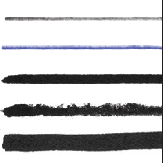
\includegraphics[width=66pt]{designspace-outline-texture}
	\vspace{-1.0\baselineskip}
\end{wrapfigure}
\noindent\textbf{Graphical Inconsistency.}
Hand-drawn strokes can vary depending on line thickness, pressure---causing a sparser
or denser texture grain and a reduced or increased color intensity respectively---as well as the type of drawing tool used.
Common drawing tools for sketching are (depicted top to bottom) graphite pencils, biros, sharpies, crayons, and markers.
The variations in grain, intensity, and thickness can be accounted for by using either image-based or procedurally-generated textures for real-time rendering.

\begin{wrapfigure}{l}{52pt}
	\vspace{-\baselineskip}
	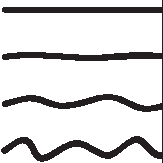
\includegraphics[width=66pt]{designspace-outline-spatial}
	\vspace{-1.0\baselineskip}
\end{wrapfigure}
\noindent\textbf{Spatial Position.}
The appearance of strokes is also determined by their straightness, 
which can be influenced  due shaking or wobbling (\emph{perturbation}) by noise. 
We use the maximum perturbation of a stroke as a control for the intensity of sketchiness \cite{Boukhelifa2012}.
For real-time rendering, 
3D spatial perturbation is implemented by subdividing  strokes (\emph{tessellation}) into multiple line segments and individually 
displacing each point by a spatially referenced offset implemented by a 3D noise texture look-up.
With the amplitude, frequency (or number of octaves), and type of noise, 
the appearance of single strokes can be further refined.
For example, white noise (high frequency) creates a highly unsettled, edgy look, 
while simplex noise causes a rather smooth and curvy appearance.
In contrast to most image-based approaches, 
our method is view-independent and produces no shower door effects. 

\begin{wrapfigure}{l}{52pt}
	\vspace{-\baselineskip}
	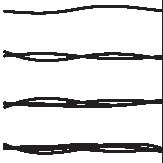
\includegraphics[width=66pt]{designspace-outline-overdraw}
	\vspace{-1.0\baselineskip}
\end{wrapfigure}
\noindent\textbf{Overdraw.}
The display of a single line is not limited to a single stroke. 
Instead, multiple strokes of the same texture but with varying perturbation can be applied (\emph{overdraw}).
We achieve this by shifting the 3D noise look-up randomly for every stroke.
Although an overdraw of strokes with varying intensities (\eg due to uneven pressure applied when drawing) allows us to increase the visualizations aesthetics, 
we do not consider it to significantly affect the perceived degree of sketchiness of outlines here.

\begin{figure*}[t!]
	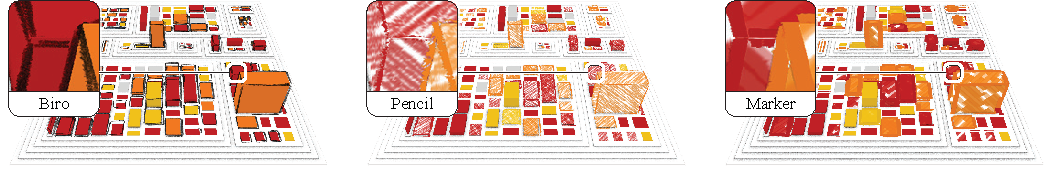
\includegraphics[width=\textwidth]{sketchiness-variations}
	\caption{Different sketchy styles: Default shading with ballpen outlines (Biro), outlines imitating colored pencils combined with slightly desaturated hatching (Pencil), thick outlines and hatches for imitating text markers (Marker).}
	\label{fig:styles}
\end{figure*}

\paragraph{Implementation.}
Sketchy outlines in 2.5D treemaps are rendered as follows: 
For all edges of all sketchy blocks an additional draw call (line draw) is dispatched.
The edges are GPU-tessellated and displaced per vertex using spatially referenced 3D offsets.
For the offsets, a single tileable, linear filtered 3D noise texture is pre-computed and scaled appropriately.
Finally, view-oriented billboards are derived along the line segments and textured via distance transformed stroke maps.
Since the number of leafs comprised by treemaps strongly varies, a level-of-detail concept as well as an appropriate effect (re)parameterization in terms of scale has not been investigated so far.

\subsection{Rendering of Sketchy Textures}
\label{subsec:surfaces}

\noindent
To render block surfaces in a sketchy style, 
we use hatch textures to modify the surface appearance such as the Pencil and Marker examples in \autoref{fig:styles}.
The design space for sketchy textures is similar to sketchy outlines; 
it includes filling style, stroke texture and stroke density.

As a replacement of solid shading in the block rendering technique, either hatching or stippling can be used.
Both convey texture, tone, and form 
by drawing closely spaced dapples or parallel as well as orthogonal strokes or stipples.
For every stroke of a texture, a homogeneous parameterization of graphical inconsistency and spatial perturbation is implied in order to maintain the blocks distinct appearance.
Varying densities of strokes might cause quite different effects---%
a cross-hatched surface displays the original color much better than a sparse hatched surface since the sparse version contains a lot more background color.
To retain the thematic mapping, hue hatching is typically used for sketchiness in information visualization \cite{Wood2012};
instead of depicting lighting and shading information, the hatching intensity indicates the degree of sketchiness (\autoref{fig:order}).

\begin{figure}[b!]
	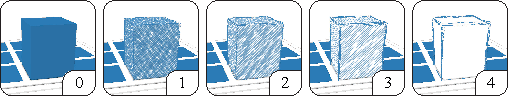
\includegraphics[width=\linewidth]{stylization-order-pencil}
	\caption{Sketchiness based on colored pencil drawing: a block can be rendered in a range from non-sketchy (left) to maximal sketchy (right). For it, the hatching intensity is designed to decrease evenly.}
	\label{fig:order}
\end{figure}

\paragraph{Implementation.}
For real-time rendering using hatching we use pre-rendered distance transformed Tonal Art Maps (\emph{TAMs}) \cite{Praun2001}.
A TAM is a set of texture images of different stroke densities, \ie hatching intensities, that get blended appropriately during fragment shading. 
Here, shower door effects are avoided by stroke-aware mipmapping.
In the case of strongly discretized color mapping---we prefer five buckets \cite{Boukhelifa2012}---a five-level sketchiness allows us to slightly account for shading without compromising its discernibility.
Similar to the setup for outlines, the TAMs' size and stroke-scales should be adjusted to the treemap size.



\section{Evaluation}
\label{sec:evaluation}

\noindent 
For the evaluation of the three sketchy rendering styles \emph{Biro}, colored \emph{Pencil}, and \emph{Marker} (\autoref{fig:styles}), we conducted a series of experiments to test their usability as a visual variable in 2.5D treemaps with focus on three aspects:
\begin{description}

	\item[Pre-study] 
	Does sketchiness as a visual variable affect the perceived height of 2.5D graphical elements in a similar way as the perceived area of 2D elements \cite{Wood2012}?
	
	\item[Study I] 
	Can the three distinct styles be processed pre-attentively (\emph{selective} characteristic)?
	
	\item[Study II]
	Are users capable of recognizing an \emph{order} when different degrees of sketchiness are depicted?
\end{description} 

\subsection{Effect on Perceived Height (Pre-Study)}
\label{sec:prestudy}

\noindent 
Since there is only sparse information on the height perception of sketched graphical elements in a 2.5D reference space, we tested for a significant effect on the height estimation of individual treemap elements when sketchiness is used (as shown for relative size estimation in 2D \cite{Wood2012}).

\textbf{Participants.}
We conducted a study with 50 participants (13 female, 37 male) aged 20 to 53 ($\mathit{M} = 27.4$, $\mathit{SD} = 7.2$) with an increased daily desktop computer usage ($\mathit{M} = 8.1$ hours, $\mathit{SD} = 2.7$) and most either strongly agreed ($n = 15$) or strongly disagreed ($n = 17$) in being experts in computer graphics and visualization on a five-value Likert scale. 

\textbf{Procedure.}
The experiment was implemented and executed as an online survey; 
the rendering styles were randomly assigned, each style having a balanced number of answers. 
First, participants were asked for their demographic information including age, gender, and PC usage per day. 
Next, two pre-answered examples showing a reference block with a higher and a shorter block in the same non-sketchy style were introduced to every participant.
\begin{wrapfigure}{l}{88pt}
	\vspace{-0.2\baselineskip}
	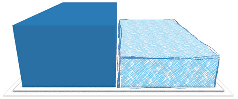
\includegraphics[width=96pt]{prestudy-example-small}
	\vspace{-2.0\baselineskip}
\end{wrapfigure}
Then, images of two blocks, one reference non-sketchy block (left) with a constant height of 100 height units (\emph{\unit{}{hu}}) and the other (right) faced with the study conditions, were shown.
The users were asked to estimate the height of the block on the right.
The input was restricted to a height range of 1 to 200.
During the study, the conditions of the actual block's height, the point of view's angle with a constant distance to the treemap center, and the rendering style varied.

\textbf{Design.}
The experiment was a 3 $\times$ 4 $\times$ 4 mixed design.
Two independent variables, angle and actual height, were tested within-subjects, while the rendering styles were tested between-subjects as follows: 
\textsl{Angle} (0$^\circ$, 15$^\circ$, 30$^\circ$), \textsl{ItemHeight} (36, 77, 132, 187), and \textsl{Style} (Solid, Biro, Pencil, Marker). 
The conditions were fully randomized for each user to prevent order and learning effects.
Aside from training, the number of estimations was 50 participants $\times $ 3 angles $ \times $ 4 heights $ = $ 600.
Each estimation results in an absolute error of the estimated height $\mathit{AbsErr} = |\mathit{ItemHeight} - \mathit{EstimatedHeight}|$, log-transformed for better readability via $\log_2(1+\mathit{AbsErr})$.

\begin{figure}[b!]
	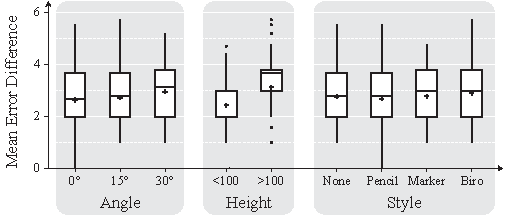
\includegraphics[width=\linewidth]{results-prestudy}
	\caption{Pre-study results depicting the mean error differences for (f.l.t.r.) angle, height, and style groups.}
	\label{fig:results-prestudy}
\end{figure}

\textbf{Results.}
We declared items as unacceptable outliers, if the estimated height was above \unit {100}{hu} as the actual block's height was below \unit{100}{hu} and vice versa.
With this constraint 5 estimates (0.01\%) were removed from the overall trials.
As expected, changing the camera angle results in significant differences (\autoref{fig:results-prestudy}, Angle) in the estimation error ($\mathit{F}_{2,76} = 17.19$, $\mathit{p} < .0001$). 
A post-hoc comparison showed that the angles 0$^\circ$ and 15$^\circ$ yield lower errors by 12\% ($\mathit{p} < .0001$) and 8\% ($\mathit{p} = .003$) respectively compared to an angle of 30$^\circ$.
The error rates \wrt the actual block heights showed significant differences: 
$\mathit{F}_{3,115} = 54.52$, $\mathit{p} < .0001$.
Besides the comparison of \unit{36}{hu} and \unit{132}{hu} ($\mathit{p} = .999$) all differences between pairs were statistically significant in a post-hoc test (all $\mathit{p} < .001$). 
In addition to looking at the four different sampled heights, we split the heights into two groups, one lower and one higher than \unit{100}{hu}.
A one-factorial Anova showed significant differences between these groups:
$\mathit{F}_{1,49} = 72.59$, $\mathit{p} < .0001$ (\autoref{fig:results-prestudy}, Height).
For the varying rendering techniques no significant difference for the height estimation errors was found: $\mathit{F}_{3,43} = .80$, $\mathit{p} < .50$ (\autoref{fig:results-prestudy}, Style).

\subsection{Pre-Attentive Processing (Study I)}
\label{sec:study-preattentive}

\noindent 
Since Biro had a bad performance in early tests---especially under the assumption of equality, \ie all elements having outlines---we focused on Marker and Pencil for pre-attentive perception and, in addition, differentiated between low and high sketchiness (\autoref{fig:order}, 1 and 3).

\textbf{Participants.}
This experiment was conducted with 24 participants (4 female, 20 male) aged 20 to 33 ($\mathit{M} = 24.9$, $\mathit{SD} = 3.4$) and having diverse background knowledge in the field of 2.5D treemaps and visualization in general.

\textbf{Procedure.}
Every participant had to perform 3 tasks (color, sketchiness, conjunction) for a specific rendering style (Marker or Pencil).
We used an eye-tracking setup to ensure that participants had to focus on a fixation cross for a
\begin{wrapfigure}{l}{88pt}
	\vspace{-0.2\baselineskip}
	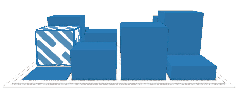
\includegraphics[width=96pt]{study1-example}
	\vspace{-2.0\baselineskip}
\end{wrapfigure}
time of \unit{700}{ms} before an image with the used visual variable was shown for maximum \unit{200}{ms} with a stimulus present or absent.
After each image, users were asked whether they recognized an element that was distinct from all others in color, sketchiness, or a conjunction of both.

\textbf{Apparatus.}
We used an eye-tracking device (EyeFollower\footnote{http://www.interactive-minds.com/eye-tracker/eyefollower} by InteractiveMinds) that allows for accurate gaze-tracking within natural head movements at a desktop environment. 
The participant was placed about \unit{60}{cm} away from a \unit{24}{inch} monitor with a FullHD screen resolution (1080p). 
Additionally, an observation monitor was placed behind a partition wall that allowed the observer to check for losses of head-tracking during the experiment.
The used software recorded gaze sample data at \unit{120}{Hz}. 

\textbf{Design.}
The experiment was a $3 \times 2 \times 2 \times 2$ mixed design with three independent variables (size, presence, sketchiness value) tested within-subjects, while the rendering styles were tested between-subjects:
\textsl{Size} (4 $\times$ 4, 7 $\times$ 7, 10 $\times$ 10), 
\textsl{Presence} (absent, present), 
\textsl{Sketchiness} (low, high),
and rendering \textsl{Style} (Pencil, Marker).
The trials started with the color task, followed by the sketchiness part and the conjunction of both.
Again, we fully randomized the variables tested within-subjects to prevent order and learning effects for \textsl{Size}, \textsl{Presence}, and \textsl{Sketchiness} for each user. 
All in all, 1728 images were shown for 24 (participants) $\times$ 3 (sizes) $\times$ 2 (present/absent) $\times$ 2 (sketchiness values) $\times$ 3 (positions) $\times$ 3 (tasks, color/sketchiness/conjunction).

\begin{figure}[b!]
	\centering
	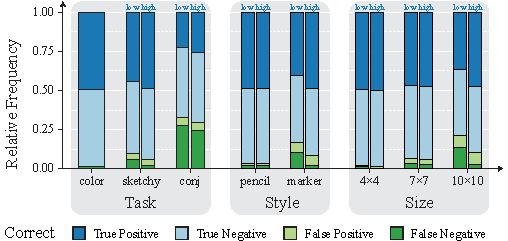
\includegraphics[width=\linewidth]{results-preattentive-study2.pdf}
	\caption{Results of Study I depicting the relative frequency for task, style, and size (low and high sketchiness).}
	\label{fig:results-study1}
\end{figure}

\textbf{Results.}
The results discussed are listed in \autoref{tab:study1-results} and shown in detail in \autoref{fig:results-study1}.
The pre-attentive processing of the visual variable color that serves as a comparative measure for our results showed a very high accuracy as well as precision and recall.
While the trials from the task of pre-attentively processing the implemented sketchiness styles also scored high values, as expected, the conjunction of both performed poorly.
Fisher's exact test significantly showed the independence by tasks ($\mathit{p}<.0005$ for I.TB, I.TS, and I.TC).
A comparison of high and low \textsl{Sketchiness} showed significant differences ($\mathit{p}=.007$ for I.SL and I.SH) with a better accuracy for high sketchiness.
Looking at the different styles, we found a significant difference in the sketchiness task ($\mathit{p}=.0002$ for I.SP and I.SM) with Pencil outperforming Marker in accuracy.
Furthermore, a significant difference between the used sizes ($\mathit{p}<.0001$ for I.S4 and I.SX) was found:
the participants' ability of pre-attentively processing sketchiness decreases as the number of elements increases.

\begin{table}[h!]%
	\caption{Results for pre-attentive processing (Study I).}
	\vspace{-0.5\baselineskip}
	\renewcommand{\arraystretch}{1.618}
	\label{tab:study1-results}
	\centering
	\small
	\begin{tabular}{lrl|lll}
		\# & \bfseries Variable & \bfseries Value & $\mathit{AC}$ & $\mathit{PC}$ & $\mathit{RC}$ \\
		\hline\hline
		I.TB 	& \textsl{Task}			& color/baseline 	& $.991$ & $.995$ & $.986$ \\
		I.TS 	& \textsl{Task}			& sketchiness 		& $.927$ & $.959$ & $.931$ \\
		I.TC 	& \textsl{Task}			& conjunction 		& $.620$ & $.904$ & $.481$ \\
		I.SL 	& \textsl{Sketchiness}	& low 				& $.905$ & $.919$ & $.889$ \\
		I.SH 	& \textsl{Sketchiness}	& high 				& $.947$ & $.925$ & $.972$ \\
		I.SP 	& \textsl{Style}		& pencil 			& $.927$ & $.986$ & $.972$ \\
		I.SM 	& \textsl{Style} 		& marker 			& $.883$ & $.932$ & $.889$ \\
		I.S4	& \textsl{Size} 		& 4 $\times$ 4		& $.991$ & $.993$ & $.993$ \\
		I.S7	& \textsl{Size} 		& 7 $\times$ 7		& $.965$ & $.951$ & $.944$ \\
		I.SX 	& \textsl{Size}			& 10 $\times$ 10 	& $.847$ & $.917$ & $.847$
	\end{tabular}
	
\end{table}

\subsection{Order of Elements (Study II)}
\label{sec:order}

\noindent
Boukhelifa et al. stated that the number of distinct levels for a sketchy rendering style is about 3 to 4 \cite{Boukhelifa2012}.
We implemented these distinct levels for all styles and conducted another study on the ability of participants to bring these levels into correct order (based on the sketchiness value).
The study was again performed as an online survey with 116 participants of whom 91 gave complete answers.

\textbf{Procedure and Design.}
Each survey included 6 sets of 5 images: an image depicting a distinct sketchiness value from non-sketchy to fully sketchy (see \autoref{fig:order}) for each of the three sketchy rendering styles of two different sizes.
The experiment was a 2 $ \times $ 3 within-subject design: 
\textsl{Size} (\emph{coarse}: 3 $ \times $ 3, \emph{fine}: 9 $ \times $ 9)
and rendering \textsl{Style} (pencil, marker). 
The number of images shown was for 91 participants $ \times $ 2 sizes $ \times $ 3 sketchy rendering styles $ = $ 546 tests.

\textbf{Results.}
For each set, a score was calculated (based on the order) representing the number of correctly answered positions, with a range from 0 (all positions wrong) to 5 (completely correct). 
A Kruskal-Wallis test showed significant differences between the rendering styles performance ($\mathit{p} < .001$, \autoref{fig:results-study2}).
A post-hoc comparison showed significant differences between Biro and Marker ($\mathit{p} = .00032$) as well as Biro and Pencil ($\mathit{p} = .00015$). 
However, we could not find this effect in the comparison between Pencil and Marker ($\mathit{p} = .72$).
The Biro style also achieved the highest score ($\mathit{M} = 4.00$, $\mathit{SD} = 1.66$), while Marker ($\mathit{M} = 3.32$, $\mathit{SD} = 1.82$) and Pencil ($\mathit{M} = 3.26$, $\mathit{SD} = 1.79$) achieved similar lower scores. 
Also, we could not find a significant difference between different sizes of images ($\mathit{p} < .001$). 

\begin{figure}[t!]
	\centering
	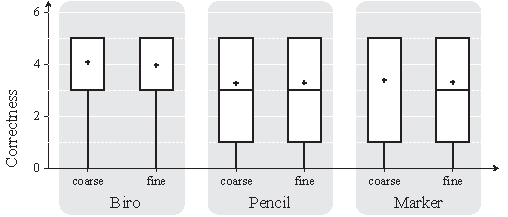
\includegraphics[width=\linewidth]{results-study2}
	\caption{Study II results depicting correctness for (f.l.t.r.) Biro, Pencil, and Marker, each in coarse and fine variation.}
	\label{fig:results-study2}
\end{figure}



\section{Conclusions and Future Work}
\label{sec:conclusion}

\noindent
Our experiments show that sketchiness can be used as an independent visual variable to map ordinal data in 2.5D treemaps without having an impact on reading and interpreting other visual variables such as color and height. 
The general weakness of sketchy rendering, 
the lowered data/ink ratio, 
is less relevant due to the uniform and regular block shape used by 2.5D treemaps---%
there is no noticeable \enquote{chart junk} \cite{Tufte1986} introduced.
Additionally, we could measure a high accuracy for the selective pre-attentive processing for 2 of 3 styles (Marker, Pencil). 
The use of a conjunction of sketchiness and color is poorly processed pre-attentively, as expected. 
In addition, the pure use of outlines (as in the Biro style) leads to poor pre-attentive processing 
and as the size of elements increases, the ability to pre-attentively process the items decreases. 
With the length of the design space of 3 to 4 distinct values as described by Boukhelifa et al., we could also show that users are able to bring depicted elements into an order 
based on their sketchiness value for all styles. 
In summary, the expressiveness of 2.5D treemaps can be extended by sketchiness as visual variable in its own right if applied to appropriate data such as ordinal data with small range. 

In future work, we would like to explore how time-varying uncertainty data can be mapped and animated in 2.5D treemaps, \eg to explore changes over time. 
We also want to explore how sketchy outlines can be integrated into a global illumination concept for 2.5D treemaps (e.g., shadow casting) and how sketchy line patterns for general ordinal data not related to uncertainty could look like.



% The preferred spelling of the word “acknowledgment” in America is without an “e” after the “g”
\section*{Acknowledgment}

\noindent
This work was funded by the Federal Ministry of Education and Research (BMBF), Germany, within the InnoProfile Transfer research group \enquote{4DnD-Vis} (\url{www.4dndvis.de}).

\bibliographystyle{plain}
{
\small
\bibliography{references}
}
\end{document}
